%% Journal of Systems and Software (JSS) manuscript
%% Based on Elsevier's elsarticle template (elsarticle-template-num.tex from
%% elsarticle.zip of April 2024), kept unmodified in ../template/.
%% elsarticle.cls, generated from the bundle with "latex elsarticle.ins", and
%% elsarticle-num.bst sit next to this file, because the submission has to
%% include every class and style that a TeX installation may lack.
%%
%% JSS guide for authors (checked 2026-10-22):
%%   - LaTeX source plus a compiled PDF. Editorial Manager accepts no
%%     subfolders, so the upload puts the figures, .cls, .bst and .bib next to
%%     main.tex; \graphicspath lets this file compile in both layouts.
%%   - a double-column layout is allowed for LaTeX submissions
%%   - abstract of at most 250 words, and 1 to 7 keywords
%%   - highlights in a separate editable file (highlights.txt), 3 to 5 bullets
%%     of at most 85 characters each, including spaces
%%   - any consistent reference style at submission (elsarticle-num)
%%   - full papers are encouraged below 18 double-column pages; a longer paper
%%     needs a justification in the submission
%%   - CRediT statement, declaration of competing interest, funding,
%%     declaration of generative AI use, and data availability with the data
%%     deposited, cited and linked (Option C); acknowledgements come directly
%%     before the references
%%   - a biography of at most 100 words per author, in an editable file
%%   - single anonymized review, so author names and repository links can stay
%% Keep the manuscript in one .tex file, without \input.
%%
%% Writing rules for the manuscript: plain words, no overclaiming, short
%% sentences, no pronouns, and no em or en dashes in the prose. Give the long
%% form of every abbreviation at first use, for example "Business Process Model
%% and Notation (BPMN)"; the abstract defines its own abbreviations. Every
%% figure, table, listing and algorithm carries a \label, and the text cites the
%% label with \ref and then discusses the content. Every entry of references.bib
%% is cited at least once.
%% Link sentences and paragraphs with explicit connectives: however, moreover,
%% furthermore, in addition, nevertheless, therefore, as a result, after that,
%% then, finally, for example, similarly, likewise, by contrast, on the other
%% hand, overall. Use a connective where a real relation exists (addition,
%% contrast, consequence, sequence, example), vary the choice, and leave plain
%% sentences where no relation needs marking.
%% Sources: the ecorefs README and evaluation notes, the two BPMN2 repositories,
%% and ../literature-review.md (every reference checked online).

%% Allow line breaks at hyphens inside long URLs in the reference list
\PassOptionsToPackage{hyphens}{url}
%% The journal layout 5p with two columns keeps the figures at the size they
%% were drawn for: one column wide, with about 8 pt lettering. The option 5p
%% also switches the preprint mode of the class off.
\documentclass[5p,times,twocolumn]{elsarticle}

%% Packages from the template (elsarticle.cls loads graphicx and natbib)
\usepackage{amssymb}
\usepackage{amsmath}
\usepackage{amsthm}

%% Packages of this manuscript
\usepackage{xcolor}
\usepackage{booktabs}
\usepackage{algorithm}
\usepackage{algorithmicx}
\usepackage{algpseudocode}
\usepackage{listings}
\usepackage[hidelinks]{hyperref}

%% The figures live in figures/ during writing and next to main.tex in the
%% Editorial Manager upload; \includegraphics names the file only.
\graphicspath{{figures/}}

%% Code listings for Java and XMI snippets. The colors match the figures:
%% blue for keywords, brown for strings and grey for comments and the frame.
\definecolor{lstkeyword}{HTML}{1C5CAB}
\definecolor{lststring}{HTML}{B8501F}
\definecolor{lstcomment}{HTML}{52514E}
\definecolor{lstframe}{HTML}{898781}
\lstset{
  basicstyle=\ttfamily\small,
  keywordstyle=\color{lstkeyword}\bfseries,
  stringstyle=\color{lststring},
  commentstyle=\color{lstcomment}\itshape,
  showstringspaces=false,
  columns=fullflexible,
  breaklines=true,
  breakatwhitespace=true,
  tabsize=2,
  frame=single,
  rulecolor=\color{lstframe},
  framesep=4pt,
  xleftmargin=4pt,
  xrightmargin=2pt,
  captionpos=b}

\theoremstyle{definition}
\newtheorem{definition}{Definition}
\theoremstyle{plain}
\newtheorem{proposition}{Proposition}

%% Drafting aid: remove every \todo before submission
\newcommand{\todo}[1]{\textcolor{red}{[TODO: #1]}}

%% The winning value of a table row or column; \boldmath also sets a
%% plus-minus sign in bold
\newcommand{\best}[1]{\textbf{\boldmath#1}}

\raggedbottom

\journal{Journal of Systems and Software}

\begin{document}

\begin{frontmatter}

\title{Towards Decentralized Model Persistence}

\author{Alfa Yohannis\corref{cor1}}
\ead{alfa.ryano@pradita.ac.id}
\cortext[cor1]{Corresponding author.}
%% Further authors: \author{Given Family} with \ead; for another institution,
%% label \author and \affiliation as in the template.

\affiliation{organization={Department of Informatics, Pradita University},
            city={Kabupaten Tangerang},
            state={Banten},
            country={Indonesia}}

\begin{abstract}
Model persistence frameworks such as the Eclipse Modeling Framework (EMF) identify a model by a location, so the content behind a reference can change unnoticed. The InterPlanetary File System (IPFS) identifies a file by a content identifier (CID) computed from the content. The paper examines the consequences for model persistence and for references between resources. An EMF resource implementation saves models to an IPFS node and loads the models by CID, and references point to fixed CIDs or mutable names. A cascade save stores every resource with a reference to a changed resource again. A small formal model states when the cascade keeps every reference current. A round trip of 11,486 real models in Business Process Model and Notation (BPMN) showed that the IPFS layer adds no failure to serialization. However, plain XML Metadata Interchange (XMI) could not store vendor extensions, and random identifiers gave the same model a new CID on every save. On 2,771 changes of acyclic reference structures from real models, the cascade gave new CIDs to exactly the affected resources and kept every reference current. Every cyclic structure kept an outdated reference, and the partitioned model of a Java code base formed one cycle of 6,934 resources. For generated models up to 10,000 elements, a save through IPFS took 40 to 43~ms longer than a save to a local XMI file, mostly because the IPFS node waited for the disk. For the largest model, the save took 12\% longer than on a network share.
\end{abstract}

%% The same bullets go to Editorial Manager as highlights.txt. The class prints
%% them on an unnumbered page before the article.
\begin{highlights}
\item An EMF resource stores models on IPFS and takes each saved content identifier as URI
\item References by content identifier pin the exact version of the target resource
\item The cascade save keeps references current on acyclic structures but not on cycles
\item A save through a local IPFS node added 40 to 43 ms, mostly waiting for the disk
\item On 11,486 real BPMN models, IPFS added no failure, while XMI and random ids did
\end{highlights}

\begin{keyword}
Model-driven engineering \sep Model persistence \sep Eclipse Modeling Framework \sep IPFS \sep Content-addressed storage \sep Cross-resource references
\end{keyword}

\end{frontmatter}

\section{Introduction}\label{sec:introduction}

Model-driven engineering (MDE) uses models to manage the complexity of platforms and to express domain concepts~\cite{schmidt2006mde}. MDE tools store models in files or in model repositories. The Eclipse Modeling Framework (EMF)~\cite{steinberg2008emf}, a software framework for implementing MDE, stores each model in a resource, and a Uniform Resource Identifier (URI) names the resource. Resources are usually serialized in the XML Metadata Interchange (XMI) format~\cite{omg2015xmi}. Common URIs such as \texttt{file://} and \texttt{platform://} name a location. The content at a location can change, but the URI stays the same. A reference to another resource therefore resolves to the current content at the location. The referenced model may have changed since the reference was created.

One example shows what the gap between a location and a version costs. A supplier and a buyer agree on a collaboration model in Business Process Model and Notation (BPMN)~\cite{omg2010bpmn}. The collaboration refers to an order process, and both models refer to a payment process of the supplier. Each reference is a file path with a fragment. Later, the supplier changes the payment process and saves the changed model at the same path. Every copy of the collaboration then resolves to the changed payment process, although the buyer agreed to the earlier version. Moreover, no reference records the agreed version, and no check reveals the change. The same three models return as a case study in Section~\ref{sec:evaluation-rq2}.

The gap appears in other modeling tasks as well. Teams keep models in shared folders or in model repositories, where several models often reference one metamodel or one shared library model~\cite{dirocco2015repositories,franzago2018collaborative}. An edit to the shared resource therefore changes the meaning of every referring model. Reverse engineering gives a second setting. MoDisco builds models of an existing code base~\cite{bruneliere2010modisco,bruneliere2014modisco}, and a later analysis should run on the same snapshot as an earlier analysis. Therefore, a model reference that names a version would remove the ambiguity in every case above.

Content-addressed storage takes a different approach. The InterPlanetary File System (IPFS) identifies content by a content identifier (CID)~\cite{benet2014ipfs,ipfsdocscid}. The CID is computed from the content, so a changed file receives a new CID~\cite{ipfsdocsipns}. Content under a given CID cannot change. In addition, any IPFS node with a copy of the content can serve it~\cite{trautwein2022ipfs}. The InterPlanetary Name System (IPNS) adds mutable names on top of CIDs~\cite{ipfsdocsipns}.

Figure~\ref{fig:settings} contrasts the two settings for a model that is split into several fragments. In a local setting, the fragments sit in a shared folder or on a repository server, and each reference names a path, so every party reads and writes the same location. In a decentralized setting, every fragment is an immutable block on IPFS, and each reference names the CID of the target. A party then fetches a fragment from any node with a copy. In addition, a mutable IPNS name marks the current version of the project.

\begin{figure*}[tbp]
\centering
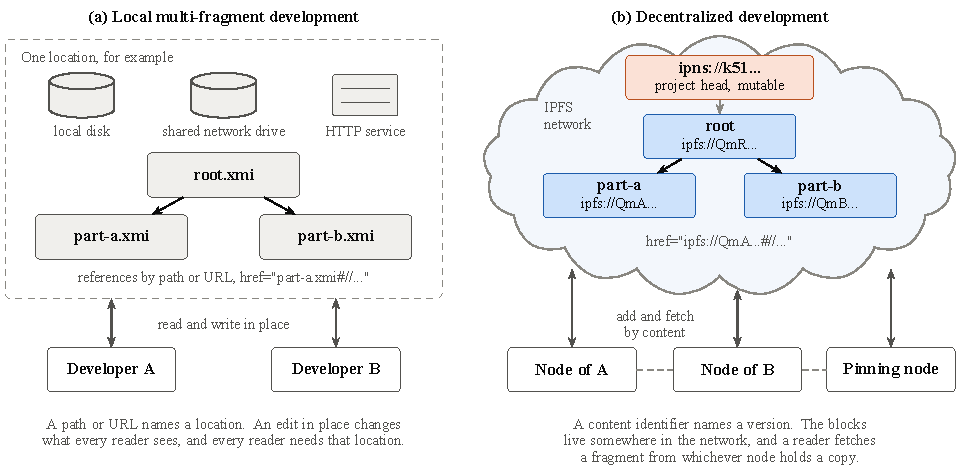
\includegraphics[width=\textwidth]{development-settings.pdf}
\caption{Development of a model that is split into fragments. (a) In a local setting, the fragments sit in one shared location, and each reference names a path. (b) In a decentralized setting, each fragment is an immutable block on IPFS, each reference names a CID, and a mutable IPNS name marks the current version of the project.}\label{fig:settings}
\end{figure*}

Content addressing has two consequences for models. First, a reference to a CID pins the exact version of the referenced model. Similarly, a lock file records the exact dependency tree of a project~\cite{npmpackagelock}, and Nix derives unique component paths from cryptographic hashes~\cite{dolstra2004nix}. Second, every save of a model creates a new CID, so references to the model need a deliberate update, and tools need to support it. Dependency updates are a known source of problems in software ecosystems~\cite{cox2019dependencies,decan2019ecosystems}. A CID is also a cryptographic hash, so a reader can check fetched content against the requested identifier on any node. However, the properties have costs. Content stays available only while at least one node stores the content. Moreover, each resource is loaded as a whole, without the on-demand loading of database-backed persistence~\cite{pagan2015repository,daniel2017neoemf}.

The properties also suggest uses outside the evaluation. A trace link, a paper or an audit can name the exact model behind a result~\cite{lamb2022reproducible}, and partners can exchange models without agreed paths~\cite{dicosmo2017heritage}.

Content-addressed persistence also brings challenges, and the paper addresses four of them. First, a resource has no identifier before the first save, and every later save changes the identifier. The persistence layer therefore needs a lifecycle that the resource model of EMF does not expect (Section~\ref{sec:rq1}). Second, a reference by CID becomes outdated as soon as the target changes. An upgrade therefore needs a cascade of saves along the referencing resources (Section~\ref{sec:rq2}). Third, a load fetches a whole resource. A large model therefore needs a split into many resources and a publication structure that keeps the parts connected (Section~\ref{sec:rq2-partitioned}). Fourth, the layer has to fit the existing EMF ecosystem, so file resources and IPFS resources share one resource set, and the editors keep the standard save and load actions (Sections~\ref{sec:rq1-differences} and~\ref{sec:tool}). The evaluation adds two challenges of the serialization (Section~\ref{sec:evaluation-rq1}). Finally, partial loading inside a single resource stays open, and Section~\ref{sec:limitations} lists the remaining limits.

Research on model persistence has mainly addressed scalability~\cite{kolovos2013roadmap}. Database-backed solutions load parts of a large model on demand~\cite{pagan2015repository,daniel2017neoemf}. Beyond scalability, model versioning systems track changes between versions of a model~\cite{koegel2010emfstore,altmanninger2009survey}. However, no reviewed approach stores EMF models on content-addressed storage (Section~\ref{sec:related}).

The paper studies content-addressed persistence for EMF with three research questions (RQ1 to RQ3):

%% Research questions adapted from the ecorefs README.md ("Research questions").
%% The README's "Publication plan" targets RQ2 at MODELS and RQ1/RQ3 at the
%% journal version; drop or shorten RQ2 here if RQ2 is published separately.
\begin{enumerate}
\item[RQ1] What are the architectural challenges of extending the persistence of EMF to content-addressed decentralized storage, and how can the challenges be addressed?
\item[RQ2] How can cross-resource references be maintained and resolved in an immutable, content-addressed environment where resource identifiers change on every modification?
\item[RQ3] What is the performance overhead of content-addressed model persistence, and under what conditions is content-addressed persistence practical for MDE toolchains?
\end{enumerate}

The paper makes four contributions:
\begin{itemize}
\item An EMF resource implementation for IPFS that saves models as XMI files on a local IPFS node and loads models by CID or IPNS name (Section~\ref{sec:rq1}). A round trip of 11,486 real BPMN models shows that the IPFS layer adds no failure to the serialization. However, plain XMI cannot store vendor extensions. Moreover, a serializer that writes random identifiers gives the same model a new CID on every save (Section~\ref{sec:evaluation-rq1}).
\item A cascade save for references by CID, with a formal model of three propositions about when the cascade keeps every reference current. On 2,771 changes of acyclic real reference structures, the cascade behaved as the propositions state. By contrast, every cyclic structure kept an outdated reference (Sections~\ref{sec:rq2} and~\ref{sec:evaluation-rq2}).
\item IPFS support in the Eclipse BPMN2 Modeler for BPMN diagrams and in the generated BPMN2 tree editor (Section~\ref{sec:tool}).
\item An evaluation of the cost against local XMI files, Git, a network share and NeoEMF, and across four IPFS nodes with emulated network delays (Section~\ref{sec:evaluation-rq3}). A case study with large MoDisco models of Java code complements the evaluation (Section~\ref{sec:evaluation-modisco}).
\end{itemize}

Section~\ref{sec:background} introduces EMF persistence and IPFS, and Section~\ref{sec:method} describes the research method. Sections~\ref{sec:rq1} to~\ref{sec:tool} present the persistence layer, the references between resources and the tool support. Section~\ref{sec:evaluation} reports the evaluation, Section~\ref{sec:discussion} answers the research questions, and Section~\ref{sec:related} covers related work before the conclusion in Section~\ref{sec:conclusion}.

\section{Background}\label{sec:background}

\subsection{Model persistence in EMF}\label{sec:background-emf}

EMF defines metamodels with Ecore. Ecore is aligned with the core subset of the Meta Object Facility (MOF), called Essential MOF~\cite{steinberg2008emf,omg2016mof}. A \texttt{Resource} holds the root objects of a model, and a URI identifies the resource. A \texttt{ResourceSet} groups resources and resolves references between the resources. A resource factory registry maps a URI scheme or a file extension to a resource factory. A \texttt{URIConverter} opens input and output streams for a URI through a list of URI handlers~\cite{steinberg2008emf}.

XMI files use the Extensible Markup Language (XML). A reference to an object in another resource is serialized as a URI with a fragment, for example \verb|href="model.xmi#//Person"|. During loading, EMF creates a proxy object for such a reference. The proxy is resolved on first access, and the target resource is loaded on demand.

\subsection{Content-addressed storage with IPFS}\label{sec:background-ipfs}

Content addressing identifies data by a hash of the data. Merkle introduced hash trees for authentication~\cite{merkle1988signature}. Later, Venti used a hash of the block contents as the identifier of a block in archival storage~\cite{quinlan2002venti}. Similarly, Git stores every object under the Secure Hash Algorithm 1 (SHA-1) checksum of its content~\cite{chacon2014progit}.

IPFS combines content addressing with a peer-to-peer network~\cite{benet2014ipfs}. Content is stored in blocks, and links between blocks form a Merkle directed acyclic graph (DAG)~\cite{benet2014ipfs}. Nodes locate content through a distributed hash table (DHT) based on Kademlia~\cite{maymounkov2002kademlia,psaras2020ipfs}. Studies describe the design and performance of IPFS~\cite{trautwein2022ipfs} and the size of the public network~\cite{henningsen2020mapping}.

A directory on IPFS also receives a CID. The directory CID covers all files in the directory. A relative path inside the directory therefore leads to the same file under the same directory CID.

IPNS provides mutable names~\cite{ipfsdocsipns}. An IPNS name is the hash of a public key. The holder of the private key can publish a new CID under the name at any time. On the other hand, resolving an IPNS name needs an extra lookup before the content can be fetched.

Kubo is an IPFS implementation in Go~\cite{kubo}. A Kubo node offers a Hypertext Transfer Protocol (HTTP) application programming interface (API). The API includes commands such as \texttt{add}, \texttt{cat}, \texttt{name/publish} and \texttt{name/resolve}.

\section{Research method}\label{sec:method}

The work follows design science. In design science, a designed artifact answers the research questions, and an evaluation of the artifact gives the evidence~\cite{hevner2004design}. The study has four steps.

The first step compares the assumptions of the EMF resource model about URIs with the properties of content addressing (Section~\ref{sec:background}). The comparison yields the five departures of Section~\ref{sec:rq1-differences}. The second step builds the artifact: the ecorefs core plugin with an EMF resource, a resource factory and a URI handler for IPFS (Section~\ref{sec:rq1}), the strategies for cross-resource references with the cascade save (Section~\ref{sec:rq2}), and two Eclipse tools with a user interface (Section~\ref{sec:tool}).

The third step validates the functions. Automated tests check save and load round trips, mixed resource sets and cross-resource references. In addition, experiments on 11,533 BPMN files from five public collections check the round trip and the determinism of the CIDs (Section~\ref{sec:evaluation-rq1}). Further experiments check the cascade save on reference structures of the same models (Section~\ref{sec:evaluation-rq2}).

The fourth step measures cost and scale. A benchmark on generated models compares saves through IPFS with saves to local XMI files. A second benchmark adds Git, a network share and a database-backed store as baselines, and a third benchmark loads models across four nodes with emulated network delays (Section~\ref{sec:evaluation-rq3}). Furthermore, a case study on large models of Java code follows the guidelines of Runeson and H\"ost~\cite{runeson2009case} and reports the publication of 1.04~GiB of models (Section~\ref{sec:evaluation-modisco}).

Each research question uses a different part of the evidence. The implementation, the functional tests and the round trip of real models answer RQ1. The reference strategies, the properties of the cascade save, the BPMN case study and the cascade experiments on real structures cover RQ2. The benchmarks and the measurements of the case studies give the numbers for RQ3. Section~\ref{sec:answers} collects the answers, and Section~\ref{sec:threats} discusses the threats to validity.

\section{Content-addressed model persistence}\label{sec:rq1}

The ecorefs core plugin adds IPFS persistence to EMF. The plugin is a Java library built with Maven for Java~11. The plugin uses the EMF Ecore library (version 2.23.0) and a Java client for the IPFS HTTP API (version 1.4.3)~\cite{javaipfsclient}.

\subsection{Architecture}\label{sec:rq1-architecture}

Figure~\ref{fig:architecture} shows the three extension points of the plugin as a Unified Modeling Language (UML) class diagram. \texttt{IPFSResourceImpl} extends the XMI resource of EMF, and \texttt{IPFSResourceFactoryImpl} creates the IPFS resources. The resource keeps the normal save of EMF and adds two saves. \texttt{saveIPFS} publishes the resource on IPFS. \texttt{saveIPFSCascaded} also publishes every resource that refers to the published resource. \texttt{IPFSURIHandlerImpl} extends the default URI handler of EMF. Every extension point talks to one local Kubo node. The enumeration \texttt{ReferenceMode} selects references by CID or by IPNS name. Finally, a fourth class, \texttt{IPFSModelPersister}, provides the cascade save behind \texttt{saveIPFSCascaded} (Section~\ref{sec:rq2-cascade}).

Listing~\ref{lst:setup} shows the configuration of a resource set. The factory is registered for the \texttt{ipfs} and \texttt{ipns} schemes. The URI handler is added at the front of the handler list, so it receives IPFS URIs before the default handlers.

\begin{figure}[tbp]
\centering
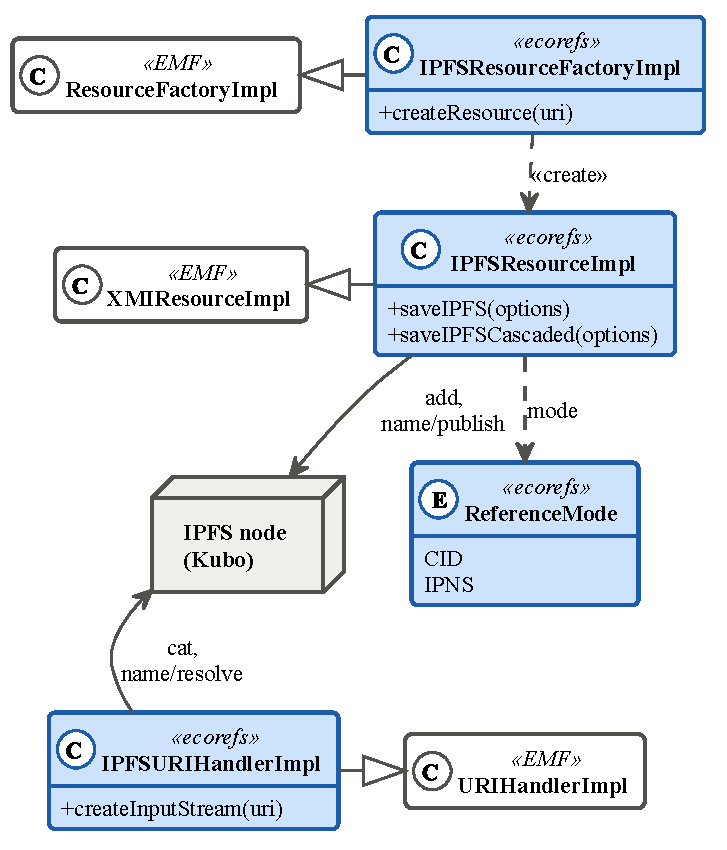
\includegraphics[width=\columnwidth]{architecture.pdf}
\caption{Unified Modeling Language (UML) class diagram of the ecorefs core plugin. Each class marked ecorefs extends one class of the EMF persistence API. The IPFS node runs Kubo and offers the HTTP API for saving and loading.}\label{fig:architecture}
\end{figure}

\begin{lstlisting}[language=Java,float=tbp,caption={Configuration of a resource set for IPFS, adapted from the test code},label={lst:setup}]
IPFS ipfs = new IPFS("/ip4/127.0.0.1/tcp/5001");
ResourceSet resourceSet = new ResourceSetImpl();
IPFSResourceFactoryImpl factory =
    new IPFSResourceFactoryImpl(ipfs);
Map<String, Object> protocols = resourceSet
    .getResourceFactoryRegistry()
    .getProtocolToFactoryMap();
protocols.put("ipfs", factory);
protocols.put("ipns", factory);
resourceSet.getURIConverter()
    .getURIHandlers()
    .add(0, new IPFSURIHandlerImpl(ipfs));
\end{lstlisting}

\subsection{Saving a model}\label{sec:rq1-save}

\texttt{IPFSResourceImpl} separates two saves. The inherited \texttt{save} is the normal EMF save, which writes the XMI to the location of the resource URI, for example a local working copy. \texttt{saveIPFS} publishes the content on IPFS instead. Figure~\ref{fig:save} shows the publication as a UML sequence diagram. A call of \texttt{saveIPFS} takes three steps. First, the resource writes the XMI serialization to a temporary file. The temporary file avoids keeping a large serialized model in memory. Second, the file is added to the local Kubo node, and Kubo pins it and returns the CID. The pin protects the file against the garbage collection of the node. Third, the resource URI is replaced with \texttt{ipfs://} followed by the CID.

In IPNS mode, the third step differs. The resource derives a key name from its URI. An Ed25519 key is created when no key with the name exists. The new CID is then published under the key, and the resource URI becomes \texttt{ipns://} followed by the key identifier. The key name is kept after the first publication, so later publications use the same name.

\begin{figure}[tbp]
\centering
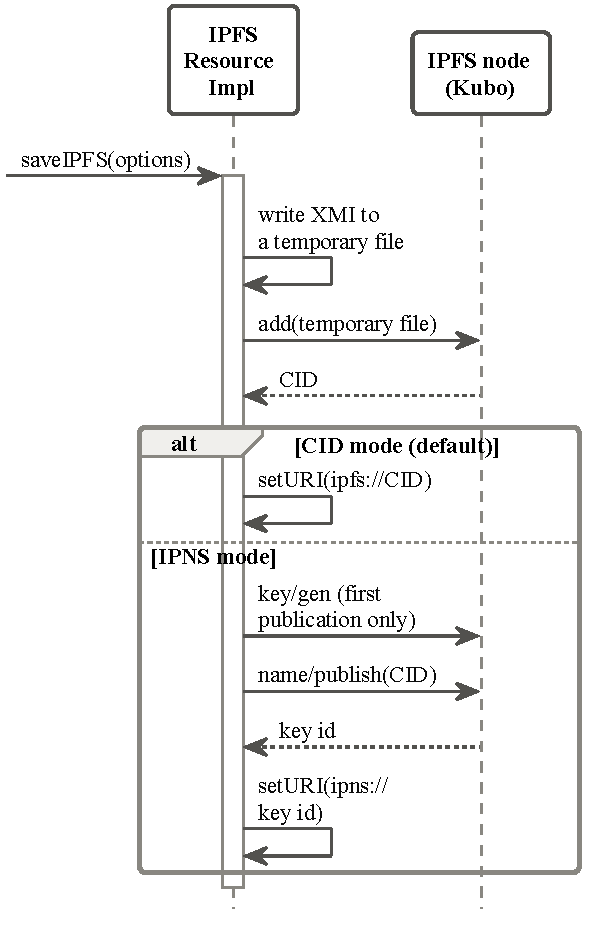
\includegraphics[width=.7\columnwidth]{save.pdf}
\caption{UML sequence diagram of \texttt{saveIPFS}, which publishes a resource on IPFS. The reference mode of the resource selects the alternative. In CID mode, the new CID becomes the resource URI. In IPNS mode, the resource URI stays an IPNS name.}\label{fig:save}
\end{figure}

\subsection{Loading a model}\label{sec:rq1-load}

\texttt{IPFSURIHandlerImpl} reads models for the resource set. For an \texttt{ipfs://} URI, the handler removes the fragment and fetches the content with the Kubo \texttt{cat} command. For an \texttt{ipns://} URI, the handler first resolves the name to a CID. The handler also reads plain \texttt{http://} and \texttt{https://} URIs. However, it rejects output streams for all four schemes. A model reaches IPFS only through \texttt{saveIPFS}, because content under an existing CID cannot change. A normal save to an \texttt{ipfs://} URI therefore fails with a message that names \texttt{saveIPFS}.

\subsection{Differences from location-based persistence}\label{sec:rq1-differences}

The implementation shows five points where content addressing departs from the assumptions of the EMF resource model:
\begin{enumerate}
\item A new resource needs a URI before the first publication, but the CID exists only after the publication. The tests and examples use placeholder URIs such as \texttt{ipfs://pending}.
\item Every publication in CID mode assigns a new URI to the resource. Code with a stored copy of the old URI still refers to the old version.
\item An output stream for an existing CID has no meaning. The resource therefore keeps the normal save of EMF for locations that accept writes. By contrast, \texttt{saveIPFS} writes a temporary file and adds the file to IPFS without the output streams of the URI converter.
\item File resources and IPFS resources can use one resource set configuration, because the IPFS handler accepts only IPFS and HTTP URIs. The test of the BPMN case study (Section~\ref{sec:evaluation-rq2}) loads local \texttt{.bpmn} files and saves IPFS resources in the same resource set.
\item A CID depends on every byte of the serialization. A location-based save may write different bytes for the same model without consequence. Under content addressing, by contrast, the same model then receives a new CID. The BPMN resource of Eclipse, for example, writes a random identifier for every element without one (Section~\ref{sec:evaluation-rq1}).
\end{enumerate}

Figure~\ref{fig:lifecycle} summarizes the resulting lifecycle as a UML state machine. In CID mode, the URI of a resource follows the content. In IPNS mode, the URI stays stable, and the IPNS name follows the content.

\begin{figure}[tbp]
\centering
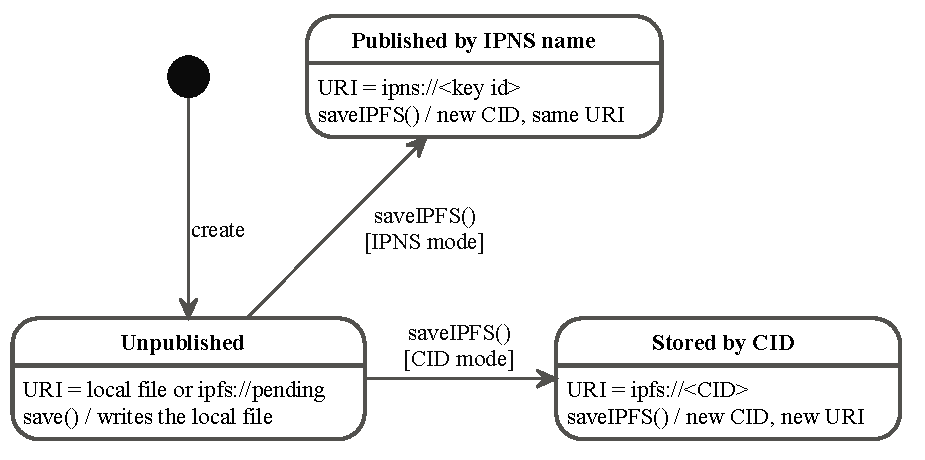
\includegraphics[width=.9\columnwidth]{lifecycle.pdf}
\caption{UML state machine of the URI of an \texttt{IPFSResourceImpl}. Each state shows the URI and the effect of a later publication after a change. Before the first publication, the normal save writes a local file. In CID mode, the URI follows the content. In IPNS mode, the URI stays the same, and the IPNS name points to the new CID. Earlier CIDs stay readable while an IPFS node stores the content.}\label{fig:lifecycle}
\end{figure}

\section{Cross-resource references}\label{sec:rq2}

\subsection{Version pinning by content addressing}\label{sec:rq2-pinning}

A reference to a resource on IPFS contains the CID of the target resource, for example \verb|href="ipfs://QmB...#//Person"|. The CID fixes the content of the target. When the target model changes, the changed model receives a new CID. The existing reference still resolves to the old version, as long as an IPFS node keeps the old content. Figure~\ref{fig:pinning} contrasts the two kinds of references.

\begin{figure}[tbp]
\centering
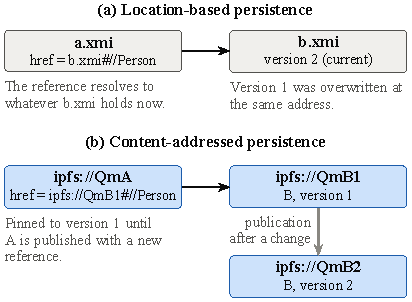
\includegraphics[width=.82\columnwidth]{version-pinning.pdf}
\caption{References under location-based and content-addressed persistence. (a) A file path resolves to the current content at the path. (b) A CID reference resolves to the version with the given CID.}\label{fig:pinning}
\end{figure}

For models developed independently, the behavior pins a dependency in the same way as a lock file~\cite{npmpackagelock,gomodules}. A model keeps working with the version used during validation. Moreover, the adoption of a newer version becomes an explicit step.

\subsection{Reference management strategies}\label{sec:rq2-strategies}

Table~\ref{tab:strategies} summarizes four strategies for references between resources on IPFS. The core plugin supports direct CID references and IPNS references through the reference mode. The publication tools for partitioned models combine directories, manifests and one IPNS name (Section~\ref{sec:rq2-partitioned}).

\begin{table*}[t]
\caption{Strategies for cross-resource references on IPFS}\label{tab:strategies}
\begin{tabular*}{\textwidth}{@{\extracolsep{\fill}}p{0.16\textwidth}p{0.30\textwidth}p{0.22\textwidth}p{0.24\textwidth}@{}}
\toprule
Strategy & Mechanism & Benefit & Drawback \\
\midrule
Direct CID references & The reference contains the CID of the target & Exact versions & Upgrades are manual \\
IPFS directories & Relative paths inside one directory with one root CID & Suits resources developed together & Any change creates a new root CID \\
IPNS indirection & The reference contains a mutable IPNS name & Resolves to the latest version & No immutability, and resolution needs an extra lookup \\
Manifest or registry & A document maps logical names to CIDs & Logical names stay stable & The manifest also needs management \\
\bottomrule
\end{tabular*}
\end{table*}

\subsection{Cascade save}\label{sec:rq2-cascade}

In CID mode, a change to one resource requires new saves of every resource with a reference to the changed resource. \texttt{saveIPFSCascaded} automates the publications (Algorithm~\ref{alg:cascade}).

\begin{algorithm}[tb]
\caption{Cascade save in CID mode}\label{alg:cascade}
\begin{algorithmic}[1]
\Procedure{CascadeSave}{$r$}
\State $X \gets$ all cross-references in the resource set
\State $A \gets \{r\}$ and every resource that reaches $r$ through $X$
\State $O \gets$ empty list
\ForAll{$a \in A$}
\State \Call{Append}{$a, A, X, O$}
\EndFor
\ForAll{$q \in O$}
\State save $q$ to IPFS
\EndFor
\EndProcedure
\Statex
\Procedure{Append}{$q, A, X, O$}
\If{$q \in O$ or $q$ lies on the current path}
\State \Return
\EndIf
\ForAll{$t \in A$ with a reference from $q$ in $X$}
\State \Call{Append}{$t, A, X, O$}
\EndFor
\State append $q$ to $O$
\EndProcedure
\end{algorithmic}
\end{algorithm}

The procedure starts with the cross-references of the resource set. A walk over the objects of each resource collects the references into other resources. The walk also counts a child that another resource stores. In addition, optional updaters of location attributes add the resources that such attributes name, for example the files of BPMN imports. From the cross-references, the procedure builds a dependency graph of the resources and collects every resource that reaches the changed resource. Next, the procedure orders the collected resources. In the order, a resource comes after every collected resource that it references. The saves then follow the order. During serialization, EMF writes the current URI of the target into each reference. The rewritten references therefore point to the new CID without any text replacement. The procedure resembles a Git commit, where a changed file leads to new tree objects up to the root~\cite{chacon2014progit}.

The order matters as soon as two reference paths reach the changed resource. In the case study of Section~\ref{sec:evaluation-rq2}, \texttt{collaboration.bpmn} refers to the order process and to the payment process, while the order process imports the payment process. A save of the collaboration before the order process would leave the collaboration with the old CID of the order process. The dependency order saves the payment process first, the order process second and the collaboration last. An earlier version of the cascade saved a resource as soon as a reference to a saved resource appeared. Moreover, the order of the saves came from a hash set, so the outcome depended on the iteration order. Figure~\ref{fig:cascade} shows the expected result for the BPMN case study of Section~\ref{sec:evaluation-rq2}. A change to \texttt{payment-process.bpmn} gives a new CID to all three resources, and every reference points to the new CID of the target.

\begin{figure}[tbp]
\centering
\begin{minipage}[t]{0.234\textwidth}
\centering
{\footnotesize (a) Before the change}
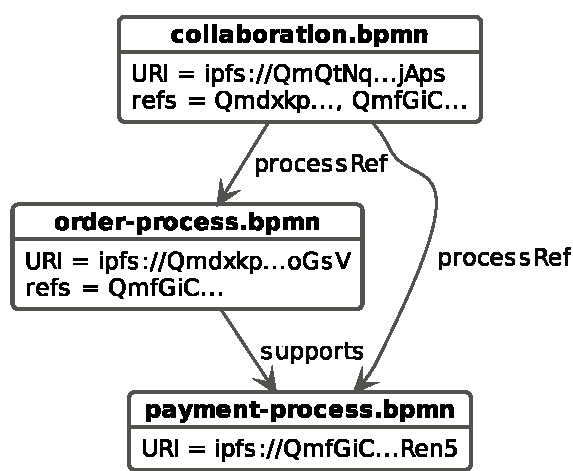
\includegraphics[width=\linewidth]{cascade-before.pdf}\\[3pt]
\end{minipage}
\hfill
\begin{minipage}[t]{0.234\textwidth}
\centering
{\footnotesize (b) After the cascade save}
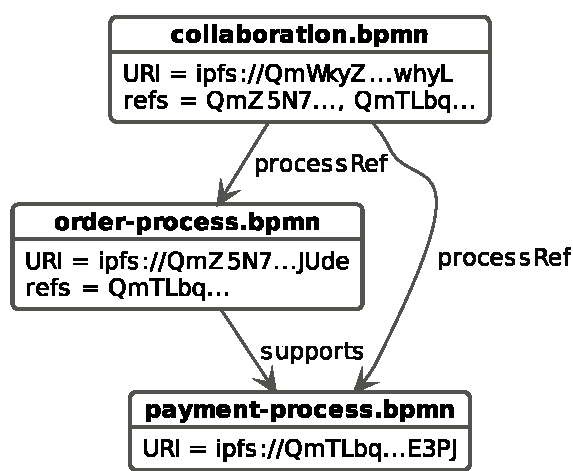
\includegraphics[width=\linewidth]{cascade-after.pdf}\\[3pt]
\end{minipage}\\[10pt]
\caption{UML object diagram of the three BPMN resources of the case study. (a) Each resource refers to the CIDs of the resources below. (b) A change to \texttt{payment-process.bpmn} and a complete cascade save give every resource a new CID. The CIDs come from the run of Section~\ref{sec:evaluation-rq2} and are shortened.}\label{fig:cascade}
\end{figure}

In IPNS mode, \texttt{saveIPFSCascaded} publishes only the changed resource. References by IPNS name resolve to the newly published CID, so the referencing resources need no new save.

Cycles need care. Resource A may refer to resource B while B refers to A. In such a cycle, one direction keeps an outdated CID in practice (Proposition~\ref{prop:cycle} in Section~\ref{sec:rq2-properties}). A test with references in both directions between two resources shows the effect. After the cascade save, one direction still names the previous CID of the other resource. \texttt{IPFSModelPublishTool} therefore checks a partitioned model for cycles before a publication in CID mode. The tool stops with an error when the resource graph contains a cycle.

\subsection{Properties of the cascade save}\label{sec:rq2-properties}

A small formal model states the properties of Algorithm~\ref{alg:cascade}. A resource set holds a finite set $R$ of resources. A snapshot $\sigma$ assigns a content $\sigma(r)$, a byte string, to every resource $r \in R$. The CID of $r$ in $\sigma$ is $\mathit{cid}_\sigma(r) = h(\sigma(r))$, where $h$ is the hash function of IPFS, by default the Secure Hash Algorithm with 256-bit values (SHA-256). The reference graph $G = (R, E)$ has an edge $(r, q)$ for $r \neq q$ in two cases. Either an object of $r$ refers to an object of $q$, or a location attribute of $r$ names $q$. In CID mode, the content $\sigma(r)$ records one CID $\rho_\sigma(r, q)$ for every edge $(r, q)$.

\begin{definition}\label{def:consistent}
A snapshot $\sigma$ is consistent when $\rho_\sigma(r, q) = \mathit{cid}_\sigma(q)$ holds for every edge $(r, q) \in E$.
\end{definition}

A save of $r$ replaces $\sigma(r)$ with a new content. The new content records the current CID of every target of $r$, and the save gives $r$ the CID of the new content. The model assumes that different contents receive different CIDs. A save therefore changes the CID of $r$ whenever it changes the content of $r$.

\begin{definition}\label{def:affected}
For a change to a resource $t$, the set $A(t)$ of affected resources holds $t$ and every resource with a path to $t$ in $G$.
\end{definition}

\begin{proposition}\label{prop:affected}
Let $\sigma$ be consistent in the sense of Definition~\ref{def:consistent}, and let a change give $t$ a new CID. A resource $r \neq t$ needs a new save for a consistent snapshot if and only if $r \in A(t)$.
\end{proposition}

\begin{proof}
Let $r \notin A(t)$, and let $(r, q) \in E$. Then $q \notin A(t)$ as well, because a path from $q$ to $t$ would extend to a path from $r$ to $t$. Saves of the resources in $A(t)$ therefore leave $q$ unchanged. The CID that $r$ records for $q$ thus stays current. Conversely, let $r \in A(t)$ with a path $r = r_0, r_1, \ldots, r_k = t$. The resource $r_{k-1}$ records the old CID of $t$, so $r_{k-1}$ needs a new save. The save changes the recorded CID and hence the content and the CID of $r_{k-1}$. The same argument then holds for $r_{k-2}$ and continues along the path up to $r_0 = r$.
\end{proof}

\begin{proposition}\label{prop:order}
Let the subgraph of $G$ on $A(t)$ be acyclic. One save of every resource in $A(t)$, each after the saves of the resources in $A(t)$ that it references, yields a consistent snapshot. Every other order with one save per resource leaves an outdated CID.
\end{proposition}

\begin{proof}
Consider the save of $r \in A(t)$, and let $(r, q) \in E$. Either $q \notin A(t)$, and $q$ keeps the same content, or $q$ was saved before $r$ and is not saved again. In both cases, the CID that $r$ records for $q$ stays current until the end. The resource $r$ is not saved again either, so every later save records the final CID of $r$. Together with Proposition~\ref{prop:affected}, every edge ends with a current CID. Conversely, if $r$ is saved before some $q \in A(t)$ with $(r, q) \in E$, the content of $r$ records the CID of $q$ from before the save of $q$. The save of $q$ then changes the CID of $q$, and the edge $(r, q)$ keeps the outdated CID.
\end{proof}

Algorithm~\ref{alg:cascade} builds such an order by a depth-first search. \textsc{Append} adds a resource only after every collected resource that it references. For an acyclic subgraph, the algorithm therefore saves every affected resource exactly once, and by Proposition~\ref{prop:affected} it saves no resource without need.

\begin{proposition}\label{prop:cycle}
Let the subgraph of $G$ on $A(t)$ contain a cycle, and let $h$ behave like a random function with $b$-bit values. Then a sequence of $n$ saves in CID mode ends in a snapshot that is consistent on the cycle with probability at most $n^2/2^b$.
\end{proposition}

\begin{proof}[Proof sketch]
Let the cycle be $r_1, r_2, \ldots, r_k, r_1$, and let it become consistent for the first time after a save of $r_1$ with content $c$. The predecessor $r_k$ then records the CID $h(c)$, and $r_k$ wrote the record before the save of $r_1$. If $h$ has never received $c$ before, $h(c)$ is a fresh random value. The value then matches the record with probability $2^{-b}$. If $c$ appeared earlier, the records around the cycle lead backwards in time. Without a collision of $h$, every resource of the cycle held the same content at an earlier time. Then $r_1$ held $c$ before the first appearance of $c$, a contradiction. A union bound over the $n$ saves and over the collisions among $n$ values gives the bound.
\end{proof}

With $b = 256$, the bound stays negligible for any realistic number of saves, so a cascade over a cycle in CID mode leaves at least one outdated CID in practice. In IPNS mode, a reference records a name, and the name does not change with the content. Cycles therefore cause no outdated references.

\subsection{Publishing partitioned models}\label{sec:rq2-partitioned}

Large models are often split into many resources. The MoDisco case study (Section~\ref{sec:evaluation-modisco}) uses one root resource and one resource per Java compilation unit. \texttt{IPFSVersionManifestPublisher} publishes such a model in four layers:
\begin{enumerate}
\item Each compilation-unit resource is an immutable file inside the directory of a component.
\item Each plug-in or module forms a component. The component directory is published as one IPFS directory with a component root CID. A component manifest lists the resources and the dependencies of the component.
\item A project version manifest records the CID of the root model and the CIDs of shared resources. For each component, the manifest records the component root CID and the CID of the component manifest.
\item One IPNS name points to the current project version manifest. A local file records the IPNS name and the CID of the current manifest.
\end{enumerate}

Figure~\ref{fig:layers} shows the layers. The layers combine three strategies from Table~\ref{tab:strategies}: directories, a manifest and IPNS indirection. Listing~\ref{lst:manifests} shows the project version manifest of the case study.

\begin{lstlisting}[language=Java,float=tb,caption={The project version manifest of the MoDisco case study, with one of 26 components. Content identifiers are shortened.},label={lst:manifests}]
{ "rootModel": {
    "path": "all-repos-merged.root.xmi",
    "cid": "Qmbu2y...Bbrmjr" },
  "sharedResources": [ {
    "kind": "aux",
    "path": "aux/orphan-types.xmi",
    "cid": "QmZQRT...hvrRdr" } ],
  "components": [ {
    "componentId":
      "eclipse.jdt.core/org.eclipse.jdt.core",
    "resourceCount": 1066,
    "componentRootCid": "QmWimK...pLy3Ms",
    "componentManifestCid": "QmaJty...SL7SS",
    "dependencyCount": 3 } ] }
\end{lstlisting}

\begin{figure}[tb]
\centering
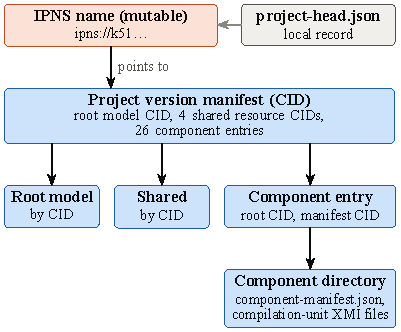
\includegraphics[width=.81\columnwidth]{publication-layers.pdf}
\caption{Publication layers of a partitioned model. One mutable IPNS name points to an immutable project version manifest. The manifest lists the CIDs of the root model, the shared resources and the component directories.}\label{fig:layers}
\end{figure} A new publication after a change to one component gives the changed component a new root CID. The other components keep the same root CIDs, because the content of the other components is unchanged. The new project version manifest is then published under the same IPNS name.

\section{Tool support}\label{sec:tool}

Two Eclipse tools bring the persistence layer to a user interface.

\subsection{Eclipse BPMN2 Modeler}\label{sec:tool-modeler}

The Eclipse BPMN2 Modeler is a graphical tool for creating and editing BPMN diagrams~\cite{bpmn2modeler,omg2010bpmn}, built with Graphiti~\cite{graphiti}. IPFS support was added to version 1.5.4 of the modeler, and the modified plug-ins target Java~17. A menu named BPMN2 IPFS publishes the current model or every model of a project, by CID or under an IPNS name. The menu also opens a model or a whole project from a CID, an IPFS path or an IPNS reference. In addition, the menu downloads a model that the current model imports, for editing. A third publish command performs the cascade of Section~\ref{sec:rq2-cascade} on BPMN imports. The command first publishes the current model. Then the command publishes, in dependency order, a new version of every model that imports the current model by CID, in the project or pinned on IPFS. The new versions differ only in the import locations. A project publication updates the imports between its models in the same way. The publication also adds a manifest in JavaScript Object Notation (JSON), which maps each relative path to a CID and names the root model. Opening the project restores the files into a new folder, or into a new project when the Project Explorer has no selection. Each project stores the Uniform Resource Locator (URL) of the Kubo API, a default load reference, the publish mode and a default IPNS key name. The modeler core also registers an IPFS URI handler, so references with \texttt{ipfs://} inside BPMN files load through Kubo.

The modeler keeps the layout of a diagram inside the BPMN file as BPMN Diagram Interchange data, so a published model carries the layout. A downloaded model goes to a folder named after its target namespace, so every version of a model lands in the same file of a project. A CID does not record the name of the published file. A model without a namespace is therefore named after its content, for example after the name of the process. IPNS publishing needs a key name that already exists in the local Kubo node.

\subsection{Generated BPMN2 tree editor}\label{sec:tool-editor}

The BPMN~2.0 metamodel of Eclipse includes a tree editor generated by EMF. The editor received a similar URI handler. The handler reads \texttt{ipfs://} and \texttt{ipns://} URIs through Kubo and rejects writes. The Kubo API URL comes from a system property, an environment variable or the default address \texttt{http://127.0.0.1:5001}. The metamodel repository with the handler builds with Maven and Tycho against Eclipse 2022-06 on Java~17. The modeler builds in the same way with Tycho~2.7.5. The build produces all 18 modules, including the core and user interface plug-ins with the IPFS commands, and an update site for installation in Eclipse. The build file of the modeler needed new repository addresses, because the original update sites of the BPMN2 metamodel, of the Graphiti milestones, of the Web Tools and of the Orbit libraries no longer exist.

\section{Evaluation}\label{sec:evaluation}

\subsection{Setup}\label{sec:evaluation-setup}

The evaluation uses generated models, real BPMN models and the Java models of the MoDisco case study. The real models come from five public collections of BPMN~2.0 files. Two collections are the test suite of the BPMN Model Interchange Working Group (MIWG) of the Object Management Group~\cite{miwgtestsuite} and the BPMN for Research collection of Camunda with models from modeling courses~\cite{camundabpmnresearch}. The other three collections are the test resources of the process engines jBPM~\cite{jbpmrepository}, Flowable~\cite{flowablerepository} and Camunda~7~\cite{camunda7repository}. The 11,533 files load into 11,486 models with the BPMN~2.0 metamodel of Eclipse, version 1.5.1, which the BPMN2 Modeler also uses. Most files carry vendor extensions, which the metamodel keeps in feature maps. RQ1 uses the files as downloaded. RQ2 uses a cleaned copy. In the copy, 1,893 files were edited until every file loads without errors. Most edits removed references to identifiers that do not exist in the file. Each experiment ran against a separate Kubo node, and the experiments did not follow references into other files or to the network.

The experiments with real models ran on a laptop with an Intel Core i7-1165G7 processor and 16~GB of memory, on OpenJDK 21.0.9. The outcomes of the experiments with real models do not depend on the speed of the machine. The timed benchmarks, by contrast, need a machine without other load. The first laptop also served for development, and earlier timed runs on the first laptop gave different times from run to run. The timed benchmarks therefore ran in one session on a second laptop without other load. The second laptop, an HP Envy, has an Intel Core i9-11900H processor (eight cores, 16 threads, up to 4.90~GHz) and 32~GB of memory and runs Ubuntu 24.04.5 with Linux 6.8.0. The HP Envy ran on mains power with the performance governor of the processor. The Java code ran on OpenJDK 21.0.12, and the plugin is compiled for Java~11. Each IPFS node ran Kubo 0.40.1 in Docker (version 29.8.2 on the HP Envy). The node of a benchmark ran in offline mode with an empty store and offered the HTTP API on the loopback interface, so the measurement covers the local store without announcements to a network. The plugin uses EMF Ecore 2.23.0, EMF XMI 2.16.0, EMF Common 2.21.0 and the Java client for the IPFS HTTP API 1.4.3, and the build uses Maven 3.9.10 on OpenJDK 17. The virtual machine of a benchmark runs with a fixed heap of 8~GB, and a garbage collection runs between the iterations, outside the measured region. The XMI copy of each benchmark model goes to a temporary file on an ext4 file system on a solid state disk. The tests measure wall-clock time with \texttt{System.nanoTime} and report milliseconds with three decimals.

\subsection{RQ1: Functional validation}\label{sec:evaluation-rq1}

The self-tests of the BPMN2 Modeler extension check reference parsing, the names given to downloaded models, command registration, bundle metadata and the documentation. An optional mode of the self-tests publishes a BPMN file to Kubo and downloads the file again. With a local Kubo~0.40.1 node, the self-tests and the round trip passed.

A round trip of the 11,486 real BPMN models of Section~\ref{sec:evaluation-setup} tests the persistence layer beyond the unit tests. Every model went through seven variants of save and load, each with a fresh load of the file and a fresh resource set for the save and for the load. Two variants store plain XMI, the format of \texttt{IPFSResourceImpl}: once in a local file and once through \texttt{saveIPFS} on the node. Two variants do the same with the EMF option for extended metadata, which lets XMI write the XML namespaces of the vendor extensions. Two further variants store BPMN~2.0 XML through the BPMN resource of Eclipse, again locally and on the node. The variant on the node adds the file in the same way as the modeler publishes a file. The seventh variant numbers every element without an identifier in document order before the BPMN save. After each load, a structural comparison checks the class, the set state and the value of every stored feature, including the entries of feature maps. A second save of a fresh load then shows whether the same model receives the same identifier. Table~\ref{tab:rq1-roundtrip} summarizes the results.

\begin{table}[t]
\caption{Round trip of 11,486 real BPMN models. Saved counts the successful saves. Equal counts the loaded models that equal the saved model. Same CID counts the models with the same CID on the second save, or with the same digest for the local file. The local file and the IPFS node gave the same outcome for every model and serialization, so each row covers both. Bold marks the best value of each column.}\label{tab:rq1-roundtrip}
\setlength{\tabcolsep}{4pt}
\begin{tabular*}{\columnwidth}{@{\extracolsep{\fill}}lrrr@{}}
\toprule
Serialization & Saved & Equal & Same CID \\
\midrule
Plain XMI & 5,505 & 2,585 & 5,505 \\
XMI with extended metadata & \best{11,484} & 0 & \best{11,484} \\
BPMN 2.0 XML & \best{11,484} & \best{10,587} & 1,850 \\
BPMN 2.0 XML, numbered ids & \best{11,484} & \best{10,587} & \best{11,484} \\
\bottomrule
\end{tabular*}
\end{table}

The IPFS layer added no failure to any serialization. For every model, the local variant and the IPFS variant of a serialization gave the same outcome. On both XMI pairs, the two variants also reported the same first difference for every model. On the BPMN pair the first difference matched for 99.2\% of the models. The other 0.8\% differ only in the random identifiers of the save.

The serialization decides the outcome instead. A plain XMI save failed for 5,981 models (52.1\%) with a null pointer exception in the XMI writer of EMF. The models hold vendor extension elements in a feature map, and plain XMI has no metadata to write the elements. Of the saved models, 2,554 lost vendor attributes such as \texttt{camunda:type} on the load, and 2,585 models (22.5\%) came back unchanged. With the option for extended metadata, all models except two saved, and the two models failed in every other variant as well. However, no model loaded back. The save writes the \texttt{definitions} element of BPMN as the root element of the XMI file. However, the XMI loader of EMF creates the matching document root only for packages that the loader creates on demand. BPMN~2.0 XML returned 10,587 models (92.2\%) unchanged. Most of the other models changed in the BPMN serializer of Eclipse, in the local file just as on IPFS. The changes were lost references to identifiers missing from the file (535 models), other lost or duplicated references (252 models), and lost mixed content or objects or failed loads (108 models).

Determinism also depends on the serializer. The XMI variants gave every model the same CID on the second save. By contrast, all 9,634 models with at least one element without an identifier received a new CID on the second BPMN save. The 1,850 other models kept the CID. The BPMN resource of Eclipse gives every element without an identifier a random universally unique identifier (UUID) during the save. After the elements were numbered in document order, every model received the same CID on both saves. The BPMN2 Modeler numbers new elements in a similar way and publishes the bytes of the saved file. The modeler therefore publishes the same CID for the same file.

Large models need a further check. The case study of Section~\ref{sec:evaluation-modisco} compares local resources with copies fetched from IPFS through EMF Compare, byte-level checks and a traversal of 4,282,694 elements. No check found a difference. Overall, the checks support the claim that a save to IPFS and a later load return the same model at the scale of the case study.

\subsection{RQ2: Reference evolution}\label{sec:evaluation-rq2}

Unit tests check the cascade on small structures: a reference from resource A to resource B, chains of two and four resources, and the diamond of Figure~\ref{fig:cascade}. After each cascade, the tests read the stored bytes of every referencing resource from the node and find the current CID of the target.

The BPMN case study of the introduction uses three real BPMN files. \texttt{payment-process.bpmn} defines a payment process with three tasks. \texttt{order-process.bpmn} imports the payment process. \texttt{collaboration.bpmn} has two participants, one for the order process and one for the payment process, and two message flows between the two processes. The references between the files use BPMN imports, and each stored file also names the CID of every imported file in the import location. A test loads the three files with the BPMN 2.0 metamodel of Eclipse, saves the three resources to IPFS and then changes the name of the payment process. On the laptop, the cascade save took 50~ms for the three saves. Figure~\ref{fig:cascade} shows the CIDs of that run before and after the change. After the cascade, the stored collaboration carries the new CID of the order process and the new CID of the payment process, and the stored order process carries the new CID of the payment process.

Two experiments check the propositions of Section~\ref{sec:rq2-properties} on reference structures of real models, from the cleaned BPMN collections. First, every model with two or more pools that run a process (1,855 models) was split into one resource per process, one resource for the collaborations with the diagrams, and one resource for the other root elements, such as messages. The split keeps every reference. A participant therefore refers to the resource of the process, a message flow to the nodes of two processes, and a diagram shape to the element of the shape. Each split model was published and then changed twice: a new name for the first process, and a new name for the first named element of the shared resource. Vendor extensions were removed before the split, because plain XMI cannot store the extensions (Section~\ref{sec:evaluation-rq1}). Second, the cleaning of the collections had removed 616 calls from a call activity to a process in another file. A script found the called file for 421 calls, and the calls became references between 538 resources, one resource per file, in 168 connected components. Every file of every component was then renamed in turn.

Each change was followed by a cascade save and three checks. First, the resources with a new CID were compared with the affected set $A(t)$ of Definition~\ref{def:affected}, which a separate scan of the stored references computed. Second, the stored bytes of every resource were read back from the node, and every \texttt{ipfs://} URI in the bytes had to name the current CID of the target. Third, a fresh resource set loaded the top resource by CID and resolved every proxy through the node. Table~\ref{tab:rq2-real} lists the outcomes.

\begin{table}[t]
\caption{Cascade saves on real reference structures: the split multi-pool models and the call graphs between files. New CIDs counts the changes after which exactly the resources of $A(t)$ received a new CID. Consistent counts the changes after which every stored reference named the current CID. Loaded counts the changes after which a load by CID resolved every proxy under the current CID.}\label{tab:rq2-real}
\setlength{\tabcolsep}{4pt}
\begin{tabular*}{\columnwidth}{@{\extracolsep{\fill}}lrrrr@{}}
\toprule
Structure & Changes & New CIDs & Consistent & Loaded \\
\midrule
Split, acyclic & 2,235 & 2,235 & 2,235 & 2,227 \\
Split, cyclic & 132 & 125 & 0 & 0 \\
Calls, acyclic & 536 & 536 & 536 & 536 \\
Calls, cyclic & 2 & 1 & 0 & 0 \\
\bottomrule
\end{tabular*}
\end{table}

The acyclic structures behaved as Propositions~\ref{prop:affected} and~\ref{prop:order} state. After every change, exactly the affected resources received a new CID, and every stored reference named the current CID. The loads by CID fetched every reachable resource under the current CID, except for eight changes in five split models. In four of the five models, a sequence flow or a data association crosses two pools in one direction. The BPMN metamodel of Eclipse declares such references without proxy resolution, so the references stay proxies after any load across resources, from IPFS or from local files.

Cycles occurred in 106 split models (5.7\%) and in one component of two files with calls in both directions. In 67 of the split models, flows cross the pools, although BPMN forbids such flows. In the other 39 models, a process refers back to the collaboration, for example through \texttt{definitionalCollaborationRef}. As Proposition~\ref{prop:cycle} predicts, no snapshot of a cyclic structure was consistent, neither after the first publication nor after a cascade. Inside a cycle, a save can also write the same bytes as an earlier save and keep the CID. Such saves are the likely cause of the seven changes of split models and the one change of a call graph whose new CIDs fell short of $A(t)$.

On the laptop, a cascade save cost about 8~ms per resource with a new CID, close to the time of storing one file with the pin on that machine (Section~\ref{sec:evaluation-rq3}). In the call graphs, the median cascade took 8.2~ms for one resource and 46.5~ms for six resources, and the typical change of a split model, with two resources, took 13.6~ms. The deepest call chain spans five files. The largest component has 31 files, and 30 of the files call the same process.

The partitioned MoDisco model of Section~\ref{sec:evaluation-modisco} shows a structure where the cascade cannot work. The serialized references of the model form one strongly connected component with all 6,934 resources. The root model lists every compilation unit, and the compilation units refer back to the root model and to the shared resources. The shared resources in turn refer to the compilation units. In CID mode, a change to any resource therefore affects all 6,934 resources, and by Proposition~\ref{prop:cycle} no cascade reaches a consistent snapshot in practice. The layered publication of Section~\ref{sec:rq2-partitioned} avoids the cascade, because the published directories keep relative paths. A change to one compilation unit gives new CIDs only to the file, to the directories above the file, to the component manifest and to the project version manifest. For the checked compilation units, the change touched 9 to 11 objects.

\subsection{RQ3: Performance}\label{sec:evaluation-rq3}

The benchmark uses generated models that consist of 100 to 500,000 elements. The models conform to a small metamodel that has only one class, \texttt{Component}. Each component has an integer identifier and can contain other components, so every model forms one tree with a single root component. For each model size, the benchmark runs three warm-up iterations and thirty measured iterations. Each iteration first copies the whole tree in memory. Every iteration changes the identifier of the root component. For example,  in iteration 5 of the model, the root component receives the identifier 5 instead of 0, while the 99 child components keep the identifiers 1 to 99. The copy therefore differs from every earlier copy, so each save stores new content with a new CID, after the edit. Next, the benchmark saves the copy to a temporary XMI file and loads the file back. After that, the same objects move from the file resource into an IPFS resource, and the benchmark saves the objects to IPFS and loads the model back by CID. The timers cover only the saves and the loads, so the copy and the new identifier stay outside the measurement. Every load also starts from a fresh resource set. Otherwise, EMF would return the objects already in memory instead of reading the file or fetching the content from the node. Tables~\ref{tab:rq3-save} and~\ref{tab:rq3-load} list the results, and Figure~\ref{fig:rq3} shows the means on logarithmic axes.

\begin{figure}[tbp]
\centering
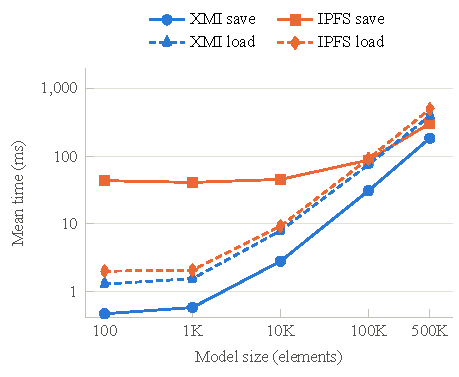
\includegraphics[width=\columnwidth]{rq3-performance.pdf}
\caption{Mean save and load times for generated models over thirty measured runs, on logarithmic axes (blue = XMI, orange = IPFS, dashed = load, solid = save). Tables~\ref{tab:rq3-save} and~\ref{tab:rq3-load} list the values.}\label{fig:rq3}
\end{figure}

\begin{table}[t]
\caption{Save times for generated models over thirty measured runs, given as mean and standard deviation. Size is the size of the serialized XMI file. Bold marks the faster save.}\label{tab:rq3-save}
\setlength{\tabcolsep}{3pt}
\begin{tabular*}{\columnwidth}{@{\extracolsep{\fill}}rrrr@{}}
\toprule
Elements & Size (MB) & XMI save (ms) & IPFS save (ms) \\
\midrule
100 & 0.004 & \best{0.46 $\pm$ 0.15} & 43.56 $\pm$ 4.45 \\
1,000 & 0.049 & \best{0.57 $\pm$ 0.21} & 41.00 $\pm$ 1.11 \\
10,000 & 0.605 & \best{2.77 $\pm$ 0.18} & 45.50 $\pm$ 0.93 \\
100,000 & 7.146 & \best{30.88 $\pm$ 1.59} & 87.83 $\pm$ 1.76 \\
500,000 & 39.566 & \best{186.15 $\pm$ 9.65} & 308.65 $\pm$ 10.92 \\
\bottomrule
\end{tabular*}
\end{table}

\begin{table}[t]
\caption{Load times for the same models over thirty measured runs, given as mean and standard deviation. Every load runs in a fresh resource set. Bold marks the faster load.}\label{tab:rq3-load}
\setlength{\tabcolsep}{3pt}
\begin{tabular*}{\columnwidth}{@{\extracolsep{\fill}}rrrr@{}}
\toprule
Elements & Size (MB) & XMI load (ms) & IPFS load (ms) \\
\midrule
100 & 0.004 & \best{1.27 $\pm$ 0.35} & 1.97 $\pm$ 0.49 \\
1,000 & 0.049 & \best{1.53 $\pm$ 0.40} & 2.05 $\pm$ 0.39 \\
10,000 & 0.605 & \best{7.86 $\pm$ 0.36} & 9.20 $\pm$ 0.89 \\
100,000 & 7.146 & \best{75.18 $\pm$ 2.57} & 92.14 $\pm$ 3.95 \\
500,000 & 39.566 & \best{399.85 $\pm$ 18.05} & 503.75 $\pm$ 21.96 \\
\bottomrule
\end{tabular*}
\end{table}

A save through IPFS took 40 to 43~ms longer than a save to an XMI file for models up to 10,000 elements. Within that range, the difference barely changed with the model size, so most of the added time is a fixed cost per save. The fixed cost is mainly the wait for the disk while the node records the pin of the saved model (Section~\ref{sec:rq1-save}). In Figure~\ref{fig:rq3}, the fixed cost appears as the flat solid orange line up to 10,000 elements. For larger models, the difference grew to 57 and 123~ms. A part that grows with the model therefore adds to the fixed cost. In relative terms, a save through IPFS took about 95 times the XMI time at 100 elements, 72 times at 1,000 elements and 16 times at 10,000 elements. For the two largest models, the ratio falls to 2.8 and 1.7. Loading from IPFS took 1.2 to 1.6 times the time of loading the XMI file. Overall, a save through IPFS is slower than a save to an XMI file, but the ratio is smaller for larger models. By contrast, a load through IPFS stays close to a load of the XMI file.

A Wilcoxon signed-rank test compares the thirty paired iterations of each model size, because the XMI file and the IPFS node receive the same content inside the same iteration. Every series gives $p < 0.001$. The matched-pairs rank-biserial correlation, the effect size of the test, is 1.00 for every save series, because the save through IPFS took longer in every pair. For loads, the correlation is 0.94 at 100 elements, 0.96 at 1,000 elements and 1.00 from 10,000 elements upward. Paired bootstrap intervals with 10,000 resamples put the added save time between 41.61 and 44.76~ms at 100 elements and between 118.46 and 126.65~ms at 500,000 elements, both at a confidence level of 95\%.

To find the cause of the fixed cost, a separate experiment measured only the step in which the node stores the file (\texttt{eval/rq3-add-probe}). A save through IPFS needs this extra step, but a save to an XMI file does not. The experiment stored the models with 100 and 10,000 elements thirty times on a fresh node and changed one factor at a time. All times are medians. With the pin, storing the smaller model took 60~ms, and without the pin, it took 1.9~ms. With the pin and with the data of the node in memory instead of on the disk, storing took 1.1~ms. The node therefore waits for the disk when it records the pin. For the model with 10,000 elements, storing took 61~ms with the pin and 4.1~ms without it, so the wait hardly changes with the model size.

Storing the smaller model with the pin took 60~ms on the HP Envy but only 8.8~ms on the first laptop, although the HP Envy has the faster processor. The disks explain the difference. To record the pin, the node waits until the disk has stored the data. Such a synchronous write of 4~KiB took 9.7~ms on the HP Envy but only 1.0~ms on the first laptop. The fixed cost therefore depends on the disk more than on the processor. Nevertheless, the implementation keeps the pin, because without it, the garbage collection of the node could delete a saved model.

A second benchmark compares the IPFS layer with three baselines on the same generated models, with the same warm-up, iterations and heap (Table~\ref{tab:baselines}). A write to \textbf{Git} saves the model in a working tree, commits the file and pushes the commit to a bare repository behind \texttt{git daemon}. A read clones the repository into a fresh folder and loads the model. A write to the \textbf{network share} saves the file through sshfs to a server on the same machine. A read loads the file through a second mount, so it cannot come from the cache of the writing mount. \textbf{NeoEMF}~\cite{daniel2017neoemf} stores the model in the embedded MapDB back end. A read of NeoEMF only opens the database and loads elements on demand, so the read together with a visit of every element is the fair comparison. Every store ran on one machine without network delay. The benchmark program ran on OpenJDK~17, because the libraries of NeoEMF do not start on Java~21. The times therefore compare the stores within the run.

\begin{table*}[t]
\caption{Mean write and read times in milliseconds over thirty measured runs per store and model size. A write lasts from the start of the save until the model is stored and shared. A read with visit lasts from the start of the transfer until every element of the loaded model was visited. Git writes with save, commit and push, and reads with clone and load. Bold marks the fastest of the four stores that share the model. The local XMI file serves as the reference.}\label{tab:baselines}
\setlength{\tabcolsep}{4pt}
\begin{tabular*}{\textwidth}{@{\extracolsep\fill}rrrrrrrrrrr@{}}
\toprule
& \multicolumn{5}{c}{Write} & \multicolumn{5}{c}{Read with visit} \\
\cmidrule(lr){2-6}\cmidrule(l){7-11}
Elements & XMI & IPFS & Git & Share & NeoEMF & XMI & IPFS & Git & Share & NeoEMF \\
\midrule
100 & 0.3 & 39.9 & 54.5 & \best{3.1} & 49.3 & 0.9 & \best{1.6} & 119.7 & 2.8 & 3.5 \\
1,000 & 0.7 & 40.4 & 56.0 & \best{4.0} & 61.0 & 1.6 & \best{2.5} & 120.7 & 3.8 & 7.0 \\
10,000 & 5.0 & 48.5 & 71.3 & \best{10.2} & 304.6 & 12.6 & \best{12.8} & 135.8 & 13.9 & 52.6 \\
100,000 & 53.3 & 109.6 & 253.9 & \best{72.2} & 3,442.9 & 123.9 & 142.7 & 276.0 & \best{132.9} & 764.6 \\
500,000 & 299.6 & 421.9 & 1,386.1 & \best{378.0} & 21,796.1 & 621.7 & 758.1 & 1,159.5 & \best{680.0} & 4,713.7 \\
\bottomrule
\end{tabular*}
\end{table*}

In the baseline run, a write through IPFS took 39.9~ms at 100 elements, against 0.3~ms for a local XMI file and 3.1~ms for the share, because the pin dominates small writes. Git needed more than 50~ms for every write and more than 115~ms for every read, because commit, push and clone each start a process. At 500,000 elements, a write through IPFS took 422~ms, 12\% longer than a write to the share (378~ms) and less than a third of a write to Git (1,386~ms). The read with visit took 758~ms through IPFS and 680~ms through the share. NeoEMF, which stores every element in the database, wrote the largest model in 21.8~s and needed 4.7~s for a read with visit. Overall, a read with visit through IPFS took at most 12\% longer than the same read from the share, while a write through IPFS paid the fixed cost of the pin. In exchange, every saved version received a fixed identifier.

The real BPMN models of RQ1 are small. The median file of a collection holds between 1.2~KB (Flowable) and 33~KB (BPMN for Research), and the largest model has 192 flow elements. Process modeling guidelines advise to split a model with more than 50 elements~\cite{mendling2010seven}. Every real model therefore lies in the range where the fixed cost dominates a save. On the laptop, adding the files to a node one by one published 166 models per second, while one add of each collection as an IPFS directory published about 1,000 models per second. Identical files received the same CID: 1,140 of the 11,533 files repeat an earlier file. However, the deduplication saved no space on disk. The node held 20,832 blocks for 10,393 distinct files, with every block in a separate file. The block store took 269~MB for 207~MB of files, against 235~MB for a plain copy in blocks of 4~KiB.

A third benchmark measures loads across nodes (\texttt{eval/multinode}). Four Kubo nodes on the HP Envy form a private network, and the Linux tool \texttt{tc netem} delays the traffic between the nodes, with round trips of about 0.2~ms without delay, 2~ms, 100~ms and 200~ms. One node saves each generated model through \texttt{IPFSResourceImpl}. Another node without any block of the model then loads it by CID through EMF. In the peered topology, the loading node keeps a connection to the saving node. In the DHT topology, the loading node finds the saving node through a provider lookup at a hub node, as a client in a public network would. Table~\ref{tab:multinode} lists the medians of thirty loads per cell.

\begin{table}[t]
\caption{Median time in milliseconds of an EMF load by CID on a node that held no block of the model, over thirty loads per cell. In the peered topology the loading node keeps a connection to the saving node, while in the DHT topology the loading node finds the saving node through a provider lookup. Bold marks the faster topology.}\label{tab:multinode}
\setlength{\tabcolsep}{4pt}
\begin{tabular*}{\columnwidth}{@{\extracolsep{\fill}}lrrrr@{}}
\toprule
& \multicolumn{2}{c}{10,000 elements} & \multicolumn{2}{c}{500,000 elements} \\
\cmidrule(lr){2-3}\cmidrule(l){4-5}
Round trip & Peered & DHT & Peered & DHT \\
\midrule
0.2~ms & \best{33} & 1,055 & \best{829} & 1,749 \\
2~ms & \best{41} & 1,078 & \best{1,147} & 2,073 \\
100~ms & \best{581} & 2,475 & \best{9,812} & 13,858 \\
200~ms & \best{1,204} & 4,018 & \best{18,325} & 26,195 \\
\bottomrule
\end{tabular*}
\end{table}

With a direct connection, the model with 10,000 elements loaded in 33~ms without delay and in 1.2~s with a round trip of 200~ms. The provider lookup added about one second without delay, because Kubo first asks the connected peers for the blocks and starts the lookup after one second. With a round trip of 200~ms, the lookup added 2.8~s. The largest model needed 18 to 26~s with a round trip of 200~ms. In the peered topology, an IPNS change became visible on another node after 31~ms without delay and after 1.24~s with a round trip of 200~ms. Through the DHT, the change took 43~ms and 1.64~s. The nodes share one host, and the emulated network loses no packets, so real networks are likely to give longer times.

\subsection{Case study: MoDisco models of Eclipse JDT}\label{sec:evaluation-modisco}

The case study uses Java models of four repositories of the Eclipse Java development tools (JDT). MoDisco reverse engineers software systems into models with MDE techniques~\cite{bruneliere2010modisco,bruneliere2014modisco}. A headless Eclipse workspace imported the Java projects of each repository. The MoDisco Java discoverer then produced one model per Java project. The resulting 39 XMI files hold 1.04~GiB with 4,282,732 XML elements and 6,315,163 serialized references to other elements. \texttt{eclipse.jdt.ui} contributes 28 models with 516~MiB, \texttt{eclipse.jdt.debug} nine models with 264~MiB, \texttt{eclipse.jdt.core} one model with 290~MiB, and \texttt{eclipse.jdt.core.binaries} one model with 10 elements. One project of \texttt{eclipse.jdt.ui} was skipped and recorded in a failure report.

The 39 models were merged into one model. A partitioner then split the merged model into one root resource and one resource per compilation unit. The partitioned model has 6,933 resources. The resources belong to 26 components, one component per plug-in or module. The components share 4 resources, and the component graph has 92 dependency edges.

The merged model was published on IPFS as one file. The partitioned model was published as one IPFS directory and through the layers of Section~\ref{sec:rq2-partitioned}.

The case study uses four kinds of checks. Byte-level checks found the published merged model, the project version manifest and the partitioned root model identical to the local files. Loader tests load the merged model and the partitioned root model, navigate into the models and resolve cross-references. A traversal test counted 4,282,694 elements in the merged model and in the partitioned resource set.

The fourth check downloads the published root model and the directories of selected components, compares the root model and the component manifests byte by byte, and compares the XMI resources of the components with EMF Compare~\cite{emfcompare}. The shared resources stay out of the comparison, because they would dominate every comparison of a single component. The byte-level checks cover them instead. Runs on selections of 4, 6 and 8 components with 44, 223 and 1,639 resources found no difference, and a recheck of the eight components on 24 March 2026 gave the same result. The largest selection holds 240.61~MiB of XMI, and the comparison took 169 to 187~s. About 90\% of the time went to the component \texttt{org.eclipse.jdt.core} with 1,066 resources.

The two forms of the model differ in load time and in traversal time. Loading the merged model took 79,982~ms, and a traversal of the loaded model took 84,304~ms. Loading the partitioned root model took 809~ms, while a traversal of the whole logical model took 380,256~ms and touched all 6,934 resources. Both traversals visited 4,282,694 elements. The partitioned form therefore suits a start on one component, and the merged form suits a scan of the whole model.

\section{Discussion}\label{sec:discussion}

\subsection{Answers to the research questions}\label{sec:answers}

For RQ1, the main challenges come from the changing identity of a resource. A resource has no final URI before the first save, the URI changes with every save, and content under an existing CID cannot be overwritten. The implementation handles the challenges with placeholder URIs and with a new URI after each save, and a read-only URI handler covers loading. A load test in a fresh resource set showed that proxy resolution works across \texttt{ipfs://} references. The round trip of 11,486 real BPMN models adds two challenges. First, the serialization has to store every model that the metamodel allows. Plain XMI failed or lost data for most models with vendor extensions, and XMI with extended metadata could not be loaded back. By contrast, the IPFS layer added no failure to the serialization. The first challenge comes from EMF and the XMI format, since the same failures occurred with local files. Second, the serialization has to write the same bytes for the same model, because random identifiers give the same model a new CID on every save. The second challenge holds for content-addressed persistence in general, since a location-based store does not depend on the bytes.

For RQ2, references by CID pin versions, and a deliberate upgrade requires new saves along the chain of referencing resources. The propositions of Section~\ref{sec:rq2-properties} state when the cascade save gives a consistent snapshot. The experiments on real structures agree with the propositions. On 2,771 changes of acyclic split models and call graphs, exactly the affected resources received a new CID, and every stored reference stayed current. Every cyclic structure kept an outdated CID. Cycles are not rare. A cycle occurs in 5.7\% of the split multi-pool models, and the whole partitioned MoDisco model forms a single cycle. For such structures, IPNS names or relative paths inside a published directory avoid the cascade, at the price of immutability or of one root CID for all resources. For the large partitioned model, component directories, manifests and one IPNS name gave a workable publication structure.

For RQ3, a save through a local Kubo node added 40 to 43~ms per model for models up to 10,000 elements, and 57~ms and 123~ms for the two largest models. Most of the fixed cost is the pin, which the node records on the disk. Loading from IPFS took 1.2 to 1.6 times the time of loading a local XMI file. The measured costs appear acceptable for interactive editing, where a save of a model with 10,000 elements took about 46~ms. Against the baselines, a write to a network share was faster than a write through IPFS at every size, and the gap shrank to 12\% for the largest model. A write to Git took 1.4 to 3.3 times as long as a write through IPFS, and a write to NeoEMF took far longer for large models. Real BPMN models are small, so their saves pay mainly the fixed cost. Across four nodes with emulated round trips of up to 200~ms, a node without the content loaded a model with 10,000 elements within 1.2~s over a direct connection and within 4.0~s through a provider lookup. An IPNS change became visible within 1.7~s.

\subsection{Comparison with Git and model repositories}\label{sec:comparison}

Git is content-addressed as well, because every object of a repository is stored under its hash~\cite{chacon2014progit}. Table~\ref{tab:comparison} therefore compares Git with the IPFS layer and with three model stores of Section~\ref{sec:related}. The main difference lies in what a reference names. A reference between two model files in Git is a path, and the path resolves to the version in the working tree. A commit pins all files of one repository together, and a submodule pins another repository as a whole. A reference by CID pins the version of one target resource in the reference itself. A model can therefore refer to an exact version of a model in another repository or organization, without a shared repository. On the other hand, Git offers history, branches and merges, which the IPFS layer leaves to manifests and IPNS names. CDO, NeoEMF and EMFStore identify model elements inside one store, so a reference names an element and not a version of a resource~\cite{cdo,daniel2017neoemf,koegel2010emfstore}. In exchange, CDO and NeoEMF load single objects on demand.

\begin{table*}[t]
\caption{Design properties of Git, three model stores and the IPFS layer of this paper.}\label{tab:comparison}
\begin{tabular*}{\textwidth}{@{\extracolsep\fill}p{0.14\textwidth}p{0.14\textwidth}p{0.15\textwidth}p{0.12\textwidth}p{0.15\textwidth}p{0.15\textwidth}@{}}
\toprule
Property & Git & CDO & NeoEMF & EMFStore & IPFS layer \\
\midrule
Identity of a version & Hash of a commit & Revision of an object in the repository & None & Version of a project & CID of a resource \\
Reference to another resource & Path in the working tree & Identifier of an object & Identifier of an object & Identifier of an element in the project & CID or IPNS name with a fragment \\
Version pinning & Per repository, submodules per repository & View on a branch or a point in time & None & Per project & Per reference \\
Partial loading & Whole files & Single objects & Single objects & Whole project & Whole resources \\
Integrity check & Hash of every object & None & None & None & CID of every resource \\
Availability & Every clone & One server & One database & One server & Every node with a copy \\
\bottomrule
\end{tabular*}
\end{table*}

\subsection{Limitations}\label{sec:limitations}

The approach loads each resource as a whole. Database-backed persistence can load parts of a model on demand~\cite{pagan2011morsa,daniel2017neoemf}, but the IPFS layer cannot. The approach also offers no query support comparable to Object Constraint Language (OCL) queries inside a database~\cite{omg2014ocl,daniel2016mogwai}. Moreover, \texttt{IPFSResourceImpl} saves plain XMI, which cannot store the vendor extensions of most real BPMN models (Section~\ref{sec:evaluation-rq1}). References that a metamodel declares without proxy resolution, such as the sequence flows of the BPMN metamodel of Eclipse, cannot cross resources at all. Furthermore, IPNS resolution needs an extra lookup and can take longer than direct CID access. A node in the public network also announces every new block to the distributed hash table, which adds work to each save. In CID mode, a change to a leaf resource causes saves along the whole dependency chain. In practice, cyclic references leave one outdated CID. CID mode is therefore unsuitable for models with references in both directions between resources, such as the partitioned MoDisco model.

\subsection{Threats to validity}\label{sec:threats}

The main threat to internal validity comes from the environment of the measurement. Garbage collection can affect single iterations. Moreover, a node in the public network announces new blocks and so competes with the next measurement. The benchmark reduces both risks with a fixed heap, a collection between the iterations, an offline node, warm-up iterations and a paired statistical test. All timed results come from one session on one machine (Section~\ref{sec:evaluation-setup}). Other disks, or the same disk at another time, can give other fixed costs. The experiments with real models add further threats. The round trip ran five virtual machines in parallel, so its times only serve as indications. The outcome of a model does not depend on the timing. RQ2 used the cleaned collections, in which 1,893 files were edited. Most edits removed references to identifiers missing from the file. Vendor extensions were removed before the split. Moreover, a script restored the calls between files by naming rules, and the rules may link a call to the wrong file of a collection. The checks of the cascade hold for the restored structures in either case.

External validity is limited by the setup. The real BPMN models from five sources widen the evidence beyond the generated metamodel. A larger collection mined from GitHub exists~\cite{turker2022bpmn}, but most files of a sample came from repositories without a license, so the evaluation used collections with known terms. The real models are small, the multi-node benchmark emulates the network on one host, and the case study covers Java code models only. Therefore, results may differ for large models of other metamodels, for real networks with packet loss and for the public IPFS network.

For construct validity, the wall-clock time of single save and load calls stands for the cost of persistence. The round trip compares stored features structurally and skips derived and transient features, which no serialization stores. In addition, the EMF Compare check covered eight components and left out the shared resources.

\section{Related work}\label{sec:related}

\subsection{Scalable model persistence}\label{sec:related-persistence}

Kolovos et al. propose a research roadmap for scalability in MDE~\cite{kolovos2013roadmap}. Morsa stores large models in a non-relational (NoSQL) database and loads model parts on demand~\cite{pagan2011morsa}. The journal version adds incremental store to the Morsa repository~\cite{pagan2015repository}. Neo4EMF provides a scalable persistence layer for EMF~\cite{benelallam2014neo4emf}. NeoEMF offers several database back ends in one framework~\cite{daniel2017neoemf}. Mogwaï translates OCL queries to Gremlin and runs the queries inside the database~\cite{daniel2016mogwai}. Scheidgen compares model representations such as XMI trees and relational data in CDO~\cite{scheidgen2013reference}. The CDO model repository stores and versions models in a central repository with relational, NoSQL or in-memory databases~\cite{cdo}. In every approach, the identifiers of model elements stay stable while the content changes.

\subsection{Model repositories and versioning}\label{sec:related-versioning}

ReMoDD collects model-driven development artifacts for research and education~\cite{france2007remodd}. Di Rocco et al. discuss model repositories for collaborative modeling, tool interoperability and model reuse~\cite{dirocco2015repositories}. EMFStore versions EMF models with operation-based change tracking, conflict detection and merging~\cite{koegel2010emfstore}. Altmanninger et al. survey version control systems for models with a focus on three-way merging~\cite{altmanninger2009survey}. Brosch et al. introduce the research challenges of model versioning~\cite{brosch2012versioning}. Model comparison supports model composition and transformation testing~\cite{kolovos2006comparison}, and EMF Compare compares and merges models of any metamodel~\cite{emfcompare}. Hawk indexes large collections of models kept in version control systems~\cite{barmpis2013hawk}. A mapping study classifies approaches to collaborative model-driven software engineering~\cite{franzago2018collaborative}. The versioning approaches record or compute differences between versions. Content addressing instead gives each version a fixed identifier derived from the content.

\subsection{Content-addressed storage outside MDE}\label{sec:related-content}

Software Heritage preserves software source code~\cite{dicosmo2017heritage}. On IPFS, InterPlanetary Wayback stores and replays web archives~\cite{kelly2016wayback}. Other work combines IPFS with blockchains for document version control~\cite{nizamuddin2019document} and for a peer-to-peer file system with content service providers~\cite{chen2017improved}. A survey compares IPFS with other decentralized data networks~\cite{daniel2022ipfsfriends}.

Decentralized collaboration on models outside MDE relies on blockchains and decentralized storage. H\"arer secures decentralized business process modeling and the tracking of process instances with a blockchain~\cite{harer2018decentralized}. Falazi et al. keep the intermediate versions of a shared deployment model on public blockchains and in decentralized storage~\cite{falazi2018blockchain}. Similarly, Tao et al. build a common data environment for building information modeling on a blockchain and IPFS~\cite{tao2021distributed}. The approaches record the versions of a model as a whole. By contrast, the present paper keeps the references between model resources inside a modeling framework and studies how the references survive new versions. Overall, no reviewed approach applies content addressing to EMF models or to references between model resources.

\subsection{Dependency management and reproducibility}\label{sec:related-dependencies}

Package managers record exact dependency versions, and the npm lock file describes the exact dependency tree for identical later installations~\cite{npmpackagelock}. Go modules record dependency versions and checksums~\cite{gomodules}. Studies show the risks of dependency updates in software ecosystems~\cite{cox2019dependencies,decan2019ecosystems}. Reproducible builds check whether binaries correspond to the source code~\cite{lamb2022reproducible}. Likewise, version pinning by CID applies the same idea to models, and a cascade save plays the role of a deliberate dependency upgrade.

\section{Conclusion}\label{sec:conclusion}

For RQ1, three extension points of EMF give a working persistence layer for IPFS, and a round trip of 11,486 real BPMN models found no failure caused by IPFS. The failures came from the serialization instead. XMI cannot store the vendor extensions of most models, and random identifiers give the same model a new CID on every save. For RQ2, references by CID pin versions. The cascade save keeps every reference current on acyclic structures. Three propositions state the property, and 2,771 changes of real structures agree with the propositions. Cycles occurred in 5.7\% of the split models and across the whole partitioned MoDisco model. A cycle keeps an outdated reference in practice, so such structures need IPNS names or published directories. For RQ3, a save through a local node added 40 to 43~ms per model up to 10,000 elements. Most of the added time is a wait for the disk while the node records the pin. For the largest model, a save through IPFS took 12\% longer than a save to a network share. Across nodes with emulated round trips of up to 200~ms, a model with 10,000 elements loaded within 4.0~s on a node without the content.

Overall, content-addressed persistence trades speed and flexibility for fixed versions. In return, a reference names the exact version of a model, any node with a copy can serve the model, and a reader can check fetched content against the CID. The costs are an added time per save, the need for deterministic serialization, deliberate upgrades of the referencing resources, and whole resources as the unit of loading.

Future work needs a serialization for IPFS resources with the vendor extensions of real models, and measurements on real networks and on the public IPFS network.

%% End matter in the order of the JSS guide for authors. Switch "the author"
%% to "the authors" if co-authors are added.

\section*{CRediT authorship contribution statement}

%% Role names follow the CRediT taxonomy verbatim.
\textbf{Alfa Yohannis:} Conceptualization, Methodology, Software, Validation, Formal analysis, Investigation, Data curation, Writing -- original draft, Writing -- review \& editing, Visualization.

\section*{Declaration of competing interest}

The author declares no known competing financial interests or personal relationships that could have appeared to influence the work reported in this paper.

\section*{Funding}

%% The guide prescribes this sentence when no funding was received.
This research did not receive any specific grant from funding agencies in the public, commercial, or not-for-profit sectors.

\section*{Declaration of generative AI and AI-assisted technologies in the manuscript preparation process}

%% Wording of the JSS guide, filled in with the earlier statement of the method section
During the preparation of this work the author used Claude Code to prototype the software, to generate the code for the MoDisco Java models, to analyse the measurement data, to draw the charts, to collect related work, and to draft and edit the text of the manuscript. The author defined the research design, the intended behavior of the system and the prompts, and the author also wrote code by hand. After using this tool, the author reviewed and edited the content as needed and takes full responsibility for the content of the published article.

\section*{Data availability}

The code, the scripts, the measurements, the generated models, the MoDisco models with the published CIDs and the cleaned BPMN collections are archived on Zenodo~\cite{yohannis2026data}. The archive leaves out the BPMN for Research collection of Camunda, because the terms of the collection do not grant redistribution. The scripts and the measurements are also in the \texttt{eval} folder of the ecorefs repository at \url{https://github.com/alfa-yohannis/ecorefs}, with one folder per experiment in \texttt{eval/results}. The BPMN2 Modeler integration is at \url{https://github.com/alfa-yohannis/org.eclipse.bpmn2-modeler-1.5.4-ecorefs}, and the BPMN~2.0 metamodel changes are at \url{https://github.com/alfa-yohannis/org.eclipse.bpmn2-ecorefs}.

\bibliographystyle{elsarticle-num}
\bibliography{references}

\end{document}
